%!TEX TS-program = xelatex
\documentclass[]{friggeri-cv}
\usepackage{afterpage}
\usepackage[]{hyperref}
\usepackage{smartdiagram}
% \usepackage[usenames, dvipsnames]{color}
\usepackage{xcolor}
\usepackage{enumitem}
\usepackage{multicol}




\setlist[itemize]{noitemsep, topsep=0pt}
\setlist[itemize]{leftmargin=*}

\hypersetup{
    pdftitle={},
    pdfauthor={},
    pdfsubject={},
    pdfkeywords={},
    colorlinks=false,       % no link border color
    allbordercolors=white,    % white border color for all
    hidelinks = true
}

\smartdiagramset{
    bubble center node font = \scriptsize,
    bubble node font = \scriptsize,
    % specifies the minimum size of the bubble center node
    bubble center node size = 0.01cm,
    %  specifies the minimum size of the bubbles
    bubble node size = 0.9cm,
    % specifies which is the distance among the bubble center node and the other bubbles
    distance center/other bubbles = 0.4cm,
    % sets the distance from the text to the border of the bubble center node
    distance text center bubble = 0.3cm,
    % set center bubble color
    bubble center node color = pblue,
    % define the list of colors usable in the diagram
    set color list = {lightgray, materialcyan, orange, green, materialorange, materialteal, materialamber, materialindigo, materialgreen, materiallime},
    % sets the opacity at which the bubbles are shown
    bubble fill opacity = 0.4,
    % sets the opacity at which the bubble text is shown
    bubble text opacity = 0.8,
}

\addbibresource{bibliography.bib}
\RequirePackage{xcolor}
\definecolor{pblue}{HTML}{0395DE}
% \definecolor{pblue}{HTML}{000080}


\begin{document}
\header{Landon}{ Wright}
      {Mechanical Engineer}

% Fake text to add separator
\fcolorbox{white}{gray}{\parbox{\dimexpr\textwidth-2\fboxsep-2\fboxrule}{
.....
}}
% In the aside, each new line forces a line break

\begin{aside}
	%\hfill \break
	\vspace{0.65 in}{~}
  \section{Telephone}
    (385) 312 2726
    ~
  \section{Mail}
    \href{mailto:landon.Wright91+resume@Gmail.com}{\textbf{Landon.Wright91@}\\gmail.com}
    ~
%   \section{Address}
%     815W 300S apt 1
%     Provo, UT 84601
%   \section{Git}
% %     \href{http://www.carminebenedetto.net}{carminebenedetto.net}
% %     \href{https://bitbucket.org/neoben}{bitbucket.org/neoben}
%     \href{https://github.com/landonbw}{github.com/landonbw}
  \section{Personal Skills}
    % 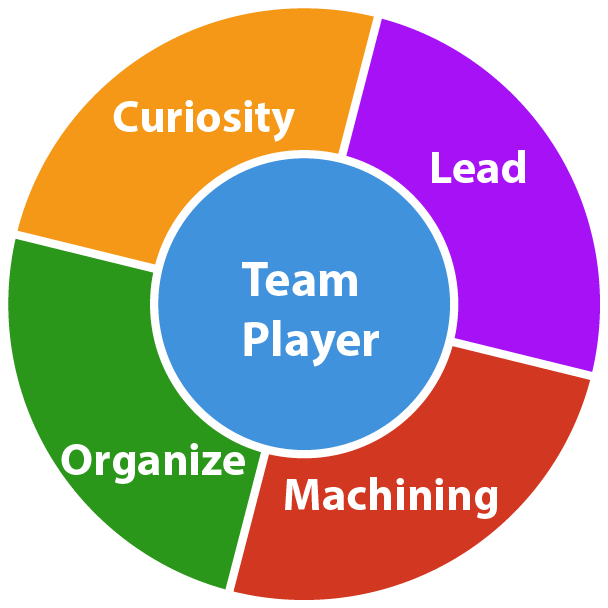
\includegraphics[width = 1.5in]{img/personalLandon.png}
%     % 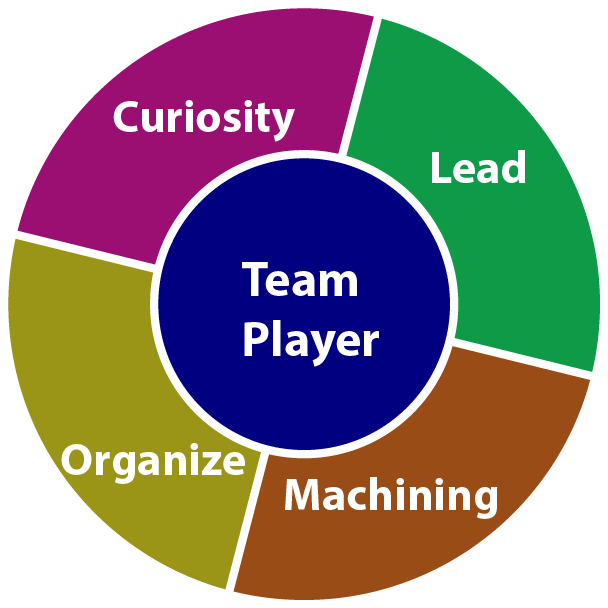
\includegraphics[width = 1.5in]{img/personalLandonDark.png}
    \smartdiagram[bubble diagram]{
        % \textbf{Team}\\\textbf{Player},
        % \textbf{Initiative},
        % \textbf{Curiosity},
        % \textbf{Problem}\\\textbf{Solving},
        % %\textbf{\vspace{2mm}Manage\vspace{2mm}},
        % \textbf{Manage},
        % \textbf{Organize}
        \textbf{Public}\\\textbf{Speaking},
        \textbf{Problem}\\\textbf{Solving},
        \textbf{Research},
        \textbf{Automation},
        \textbf{Leadership},
        \textbf{Hard}\\\textbf{Work}
    }
%     ~
    ~
    \section{CAD Preference}
    \textbf{NX}
\includegraphics[scale=0.40]{img/4stars.png}
    \textbf{Solidworks}
\includegraphics[scale=0.40]{img/3stars.png}
    \textbf{Fusion 360}
\includegraphics[scale=0.40]{img/3stars.png}
    % \textbf{Creo}
\includegraphics[scale=0.40]{img/1stars.png}
    ~
    \section{Programming}
%    \vspace{1mm}
    % 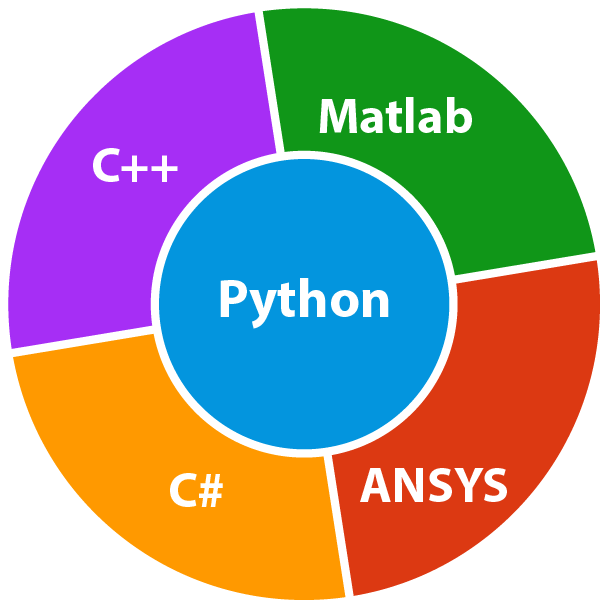
\includegraphics[width = 1.5in]{img/programmingLandon.png}
    % 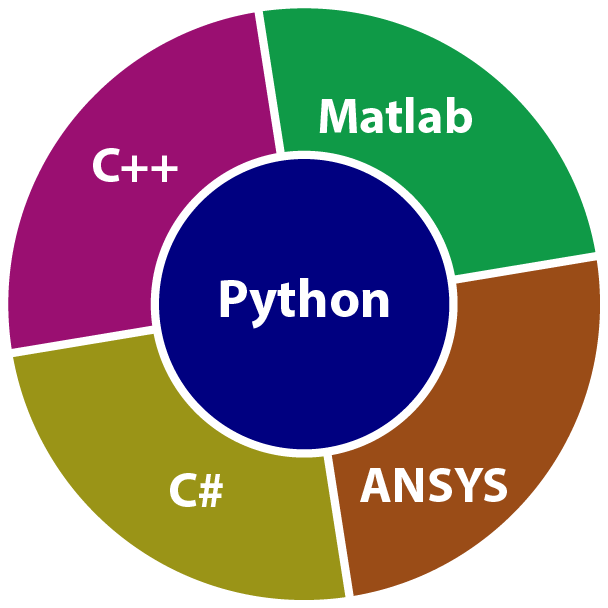
\includegraphics[width = 1.5in]{img/programmingLandonDark.png}
    \smartdiagram[bubble diagram]{
      \textbf{Python},
      \textbf{C/C++},
      \textbf{Matlab},
      \textbf{C\#},
      \textbf{ANSYS}\\\textbf{APDL},
      \textbf{Julia},
      \textbf{JSL\vspace{-4mm}}

      %\textbf{}
}
    ~
    \section{Languages}
    \textbf{English}
\includegraphics[scale=0.40]{img/5stars.png}
    \textbf{Spanish}
\includegraphics[scale=0.40]{img/3stars.png}
    ~
    \section{Certifications}
    Amateur Extra HAM
    GO PLM for NX
    ~
\end{aside}

\section{Education}
\vspace{-3mm}
\begin{entrylist}
    \entry
    {09/17 - 04/19}
    {Master of Science, Mechanical Engineering}
    {BYU, Provo UT}
    {GPA: 3.85\\Relevant Coursework: Multi-Agent Systems, Statistical Methods for Research, \textbf{Optimization Techniques}, Systems Engineering and CAD Applications Computer Aided Engineering Software Development}

    \entry
    {01/12 - 04/17}
    {Bachelor of Science, Mechanical Engineering}
    {BYU, Provo UT}
    {Relevant Coursework: \textbf{Flight Dynamics and Control}, Mechanical Systems Design Applications, Engineering Measurements}



\end{entrylist}



\vspace{-4mm}

\section{Skills and Abilities}
\vspace{-3mm}
\begin{entrylist}

    % \entry
    % {}
    % {Computer Aided Design (CAD)}
    % {}
    % {\vspace{-4mm}
    % \begin{itemize}
    %     \item (Fusion) Recognized by Autodesk with two \$250 awards for excellence in part modeling
    %     \item (Fusion/solidThinking Inspire) Designed, optimized and fabricated bike rack support mounts
    %     % \item (Solidworks)  Created suite of parametric models to allow for rapid generation of customized parts to suit client needs
    %     \item (NX) Three years experience modeling aerospace components to evaluate performance of advanced CAD applications
    % \end{itemize}\vspace{1mm}}


    % \entry
    % {}
    % {Computer Programming}
    % {}
    % {\vspace{-4mm}
    % \begin{itemize}
    % \item (C\#) Contributed to development of over 50,000 lines of code interfacing with the NX API
    % \item (Python) Created control systems, simulations, and animations of various mechanical systems to evaluate effectiveness of proposed control algorithms
    % \item (Julia) Working to develop agent-based model of autonomous vehicle adoption rates under variations in public policy
    % \end{itemize}\vspace{1mm}}


    % \entry
    % {}
    % {Statistical Analysis}
    % {}
    % {\vspace{-4mm}
    % \begin{itemize}
    % \item (JMP) Determined which environmental factors have the largest impacts on webbing strength (Best new research ITRS 2017)
    % \item (JMP) Co-presenter at the 2017 JMP Discovery Summit demostrating statistical analysis of flight simulator created in JSL (Best paper runner-up)

    % % \item (JMP) Analyzed statistical patterns in randomized experiments to determine factors that contribute to decreases in webbing breaking strength.

    % %\item (JMP) Analyzed environmental factors that effect webbing strength in Search and Rescue applications -  Awarded best new research ITRS 2017


    % % \item (Python/JMP) Predicted car values to within \$4000 through market tracking and analysis of over 100,000 car advertisements
    % \end{itemize}\vspace{1mm}}

    % \entry
    % {}
    % {Communication}
    % {}
    % {\vspace{-4mm}
    % \begin{itemize}
    % \item Awarded best new research for work presented at the 2017 International Technical Rescue Symposium
    % % \item Defined and oversaw progress towards achievement of technical and social constraints in development of products for tea packaging process in Peru
    % % \item Presented actionable results of academic research to volunteers and industry professionals at the 2017 International Technical Rescue Symposium
    % \item Co-presenter at the 2017 JMP Discovery Summit demonstrating statistical analysis of flight simulation statistics in JSL (Best Paper runner-up)
    % \end{itemize}\vspace{1mm}}


    \entry
    {}
    {Control Systems}
    {}
    {\vspace{-4mm}
    \begin{itemize}
        \item (Python) Created flight simulator and aircraft control systems for Micro Air Vehicles including PID control, total energy control, and Kalman filters and path planning algorithms
        \item (Python) Implemented PID, State Space, and Loop Shaping control methods for a two rotor "Whirlybird"
    \end{itemize}
    \vspace{1mm}}








    \entry
    {}
    {Leadership}
    {}
    {\vspace{-4mm}
    \begin{itemize}
    % \item Coordinated up to 10 students in verification testing of innovative multi-user CAD software
    % \item Team
    \item Mentored a team of 3 students with \$50,000 budget to investigate CAD automation methods leading to a publication in CAD and Applications Journal
    \item Prepared and presented project updates to multinational aerospace and automotive corporations to secure future funding for research activities
    % \item Led group of 12 students in modeling of wing structure for original Wright Flyer
    \end{itemize}\vspace{1mm}}




    % \entry
    % {}
    % {Research}
    % {}
    % {\vspace{-4mm}
    % \begin{itemize}
    % \item Initiated novel research into development of a CAD model taxonomy
    % % \item Coordinated with corporate sponsors to obtain funding for research projects involving collaborative CAD tools
    % \item Received corporate support for research regarding mechanical advantage of rappel devices
    % \item Received university funding to research and present the effect of environmental factors on the strength of climbing webbing
    % \item Awarded Best New Research at International Technical Rescue Symposium 2017
    % % \item Used JMP statistical package to analyze statistical effect of environmental factors on webbing strength
    % \end{itemize}\vspace{1mm}}

    \entry
    {}
    {Product Development}
    {}
    {\vspace{-4mm}
    \begin{itemize}
        \item Recognized by Associate Administrator of National Nuclear Security Administration for excellence in design of nuclear ordinance tooling
        \item Designed and constructed an adhesive free paper sealing device used to reduce tea bag packaging time by 85\%
    \end{itemize}
    \vspace{1mm}}


    % \entry
    % {}
    % {Prototype and Equipment Construction}
    % {}
    % {\vspace{-4mm}
    % \begin{itemize}
    % % \item Designed and constructed paper sealing device to improve productivity of a tea packaging factory in Peru
    % % \item Built and flew an RC aircraft in order to validate engineering calculations predicting flight characteristics
    % \item Manufactured equipment to allow for the use of minimum quantity lubrication on an existing horizontal machining center
    % \item Developed and built a testing apparatus in order to accurately measure the mechanical advantage of rappel devices
    % \item Constructed Large scale cutaway of a lock cylinder and key in order to teach elementary school students how locks and keys function together
    % % \item Oversaw design and construction of large scale kaleidoscope to support a university artist in the development of her final show for the Utah Museum of Contemporary Art.
    % \item Designed equipment to safely lift and transport nuclear ordnance of varying size.
    % \end{itemize}
    % \vspace{1mm}}




    % \entry
    % {}
    % {Finite Element Analysis}
    % {}
    % {\vspace{-4mm}
    % \begin{itemize}
    %     \item Created parametric models for analysis of various geometries and loading conditions in ANSYS
    %     \item Developed ANSYS models for static stress, large deflections, modal analysis, buckling and other failure modes
    % \end{itemize}
    % \vspace{1mm}}





\end{entrylist}


\vspace{-4mm}








\section{Experience}
\vspace{-3mm}
\begin{entrylist}
  \entry
    {05/18 - 08/18}
    {Systems Engineer Intern}
    {Honeywell, Phoenix, UT}
    {\vspace{-4mm}
    \begin{itemize}
        \item (MATLAB) Reduced circuit analysis time from three days to three hours with a 98\% reduction in rework time through programmatic automation
        \item Elemenated redundant test methods by evaluating and comparing competing requirements of RTCA DO-160, MIL-STD-810, and MIL-STD-461.
        \item Prepared and presented critical design review slides to customer
    \end{itemize}\vspace{1mm}}

  \entry
    {02/14 - Now}
    {Research Assistant}
    {BYU XDL, Provo, UT}
    {\vspace{-4mm}
    \begin{itemize}
        % \item Planned and carried out user testing to evaluate the effectiveness of advanced and experimental CAD tools
        \item Co-founded Search and rescue arm of research leading to best new research award at the 2017 International Technical Rescue Symposium
        \item (C\#) Team lead of group developing algorithms to create simplified assembly representations for reduced CAD software load times
        \item (C\#) Developed and debugged multi-user collaborative CAD software
        % \item (C++/OpenCV) Designed tools to analyze mouse movement and error messages in screen recordings
    \end{itemize}\vspace{1mm}}
    % {Worked with Boeing and other aerospace partners to secure funding, develop, and test collaborative CAD applications based in Siemens NX\\}
%   \entry
%     {04/16 - Now}
%     {Developer}
%     {BYU Cad Lab, Provo, UT}
%     {Contributed to development of advanced CAD components in C\#\\}
%   \entry
%     {02/14 - 04/16}
%     {Tester Lead}
%     {BYU Cad Lab, Provo, UT}
%     {Organized testing team in performace validation of revolutionary multi-user CAD package (NX-based)\\}
%   \entry
%     {04/16 - 09/16}
%     {Research Assistant}
%     {Compliant Mechanisms Research Laboratory, Provo, UT}
%     {\vspace{-4mm}
%     \begin{itemize}
%         \item Implemented technology push product design methods to discover novel applications of origami inspired compliant mechanisms
%         \item Created a process to manufacture textiles with shape memory
%     \end{itemize}\vspace{1mm}}
    % {Investigated possible techniques to apply origami inspired compliant mechanisms to manufacturing processes\\}

  \entry
    {04/15 - 09/15}
    {Engineering Intern}
    {Precorp Inc, Spanish Fork, UT}
    {\vspace{-4mm}
    \begin{itemize}
        % \item Analyzed function and purpose of pyrophyllite in synthetic diamond production in order to propose materials with an annual cost saving of \$100,000
        \item Generated a cost savings of \$100,000 annually by evaluating alternatives to pyrophyllite in poly-crystalline diamond production
        \item Developed qualification tests for the evaluation of pyrophyllite substitutes
        \item Investigated methods of non-destructive crack detection in poly-crystalline diamond to eliminate time intensive manual inspection
     \end{itemize}\vspace{1mm}}
    % {Improved manufacturing and inspection techniques for polycrystalline diamond cutting tools used in the aerospace and automotive industries}
    % \entry
    % {Ongoing}
    % {Personal Projects}
    % {Projects completed while student at BYU}
    % {\vspace{-4mm}
    % \begin{itemize}
    %     \item Initiated, obtained funding, carried out, and presented research on the impact of environmental factors on climbing webbing strength
    %     \item Designing computer vision based CNC honey dispensing device
    %     \item (Fusion/solidThinking Inspire) Designed, optimized and fabricated bike rack support mounts

    % \end{itemize}\vspace{1mm}}
\end{entrylist}

% \section{Awards}
% \vspace{-5mm}
% \begin{multicols}{2}
%     \begin{itemize}
%         \item Capstone project recognized as outstanding design by the National Nuclear Security Administration
%         \item Best new research ITRS 2017
%     \columnbreak
%         \item thing 2
%     \end{itemize}
% \end{multicols}
% ~
~
\end{document}
